\documentclass[
	11pt,
	aspectratio=169,
]{beamer}

% Setting the colors
\hypersetup{
	colorlinks,
	citecolor=cyan,
	linkcolor=.,
	urlcolor=cyan
}
\usepackage[utf8]{inputenc}
\usepackage[T1]{fontenc}

% Remove these 2 lines
\usepackage[english]{babel}
\usepackage{blindtext}

% Defining a color
\usepackage{xcolor}
\definecolor{uwo-purple}{HTML}{4F2683}
\definecolor{uwo-gray}{HTML}{807F83}

% Refs
\usepackage[backend=bibtex,style=alphabetic]{biblatex}
\addbibresource{refs.bib}

% Phonetic characters
\usepackage{tipa}
\usepackage{tipx}



\usetheme{CambridgeUS}

% Customizing the template
\setbeamercolor{frametitle}{fg=uwo-purple}
\setbeamercolor{title}{fg=uwo-purple}
\setbeamercolor{palette primary}{fg=black, bg=uwo-purple!30!white}
\setbeamercolor{palette secondary}{fg=black, bg=uwo-purple!20!white}
\setbeamercolor{palette tertiary}{bg=uwo-purple}


\begin{document}
	\author{Amir HaghighatiMaleki}
	\title{Design/Cybernetics: Two Sides of One Coin}
	\subtitle{Reading Course Presentation}
	\logo{
\includegraphics[width=0.7cm]{resources/uwo-purple.png}}
	\institute{Insight Lab}
	\date{\today}
	\subject{Reading Course Presentation}
	%\setbeamercovered{transparent}
	%\setbeamertemplate{navigation symbols}{}
	\begin{frame}
		\maketitle
		\centering\tiny\hyperlink{http://insight.uwo.ca}{insight.uwo.ca}\\
		\centering\tiny\hyperlink{mailto:ahaghig3@uwo.ca}{ahaghig3@uwo.ca}
	\end{frame}

\begin{frame}
	\textit{\rm``The progress of knowledge is at the same time the progress of ignorance.''}\\
	--- Edgar Morin \cite{morin_1992} \\
	\vspace{0.4cm}
	\textit{\rm``The very act of focusing prevents us from seeing.''}\\
	--- ?? \\
	\vspace{0.4cm}
	\textit{\rm``We do not see what we do not see, and what we do not see does not exist.''}\\
	--- Humberto R. Maturana and Francisco J. Varela \cite{maturana_varela_1987}\\
	\vspace{0.4cm}
	\textit{\rm``The only way to overcome second-order deficiencies is with therapies of second order.''}\\
	--- Heinz von Foerster \cite{vonFoerster_2003}\\
	\vspace{0.4cm}
	\begin{figure}
		\centering
		\href{https://anewage.github.io}{
			
\includegraphics[width=2cm]{resources/anewage_github_io.png}
		}
	\end{figure}
\end{frame}

\section*{Prolouge}
\begin{frame}
	\frametitle{Prologue I}
	\begin{columns}
		\column{0.3\textwidth}
			\begin{figure}
				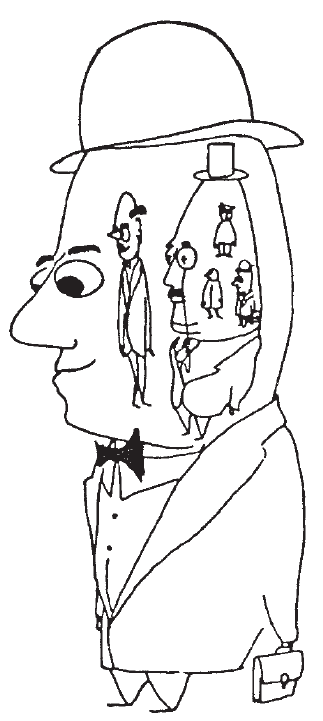
\includegraphics[height=0.7\textheight]{resources/man.png}
			\end{figure}
		\column{0.3\textwidth}
			\begin{figure}
				
\includegraphics[width=\textwidth]{resources/liar.jpg}
			\end{figure}
		\column{0.3\textwidth}
			\begin{figure}
				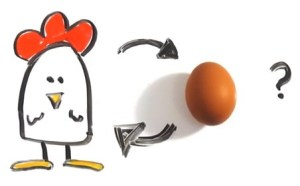
\includegraphics[width=\textwidth]{resources/chickenegg.jpg}
			\end{figure}
	\end{columns}
\end{frame}

\begin{frame}
\frametitle{Prologue II}
	{\textbf{Gödel's incompleteness} theorems can be summarized as: \\
		It is impossible to construct a theoretical language that will not \textcolor{teal}{close on itself}, with the result that there are statements that are \textcolor{teal}{undecidable} in that language.} \\
	\vspace{0.5cm}
	{In other words: There are things that you \textcolor{teal}{cannot explain within a paricular language}.}
	
\end{frame}

\section*{Overview}
	\begin{frame}
		\frametitle{Agenda}
		\tableofcontents
	\end{frame}

\section{Introduction}
	\subsection{Definitions}
		\begin{frame}
%			\setbeamercovered{transparent}
			\frametitle{Definition(s) of Cybernetics}
			\framesubtitle{The Root of the Word}
			\textbf{Cybernetics} (\textbackslash \textipa{saI\texttt{}b@r"netIks}\textbackslash):
			\begin{itemize}
				\item<1-> From Greek `kybernetes': `\textcolor{teal}{steersman}', `kybernan': `to steer or pilot a ship, direct as a pilot'
				\item<2-> Is about having a goal and taking action to achieve that goal
				\item<3-> The art of steering \cite{pangaro_web}:
			\end{itemize}
			\centering\includegraphics<3>[width=7.2cm]{./resources/steering1.png}
			\centering\includegraphics<4>[width=7.2cm]{./resources/steering2.png}
			\centering\includegraphics<5>[width=7.2cm]{./resources/steering3.png}
			\centering\includegraphics<6>[width=7.2cm]{./resources/steering4.png}
			\centering\includegraphics<7>[width=7.2cm]{./resources/steering5.png}
			\centering\includegraphics<8>[width=7.2cm]{./resources/steering6.png}
			\centering\includegraphics<9>[width=7.2cm]{./resources/steering7.png}
			\centering\includegraphics<10>[width=7.2cm]{./resources/steering8.png}
			\centering\includegraphics<11>[width=7.2cm]{./resources/steering9.png}
			\centering\includegraphics<12>[width=7.2cm]{./resources/steering10.png}
		
%			\setbeamercovered{invisible}
		\end{frame}
		\begin{frame}
			\setbeamercovered{transparent}
			\frametitle{Definition(s) of Cybernetics (Cont'd)}
			\framesubtitle{Soooo... What is Cybernetics?}
			\begin{itemize}
				\item<1->Ship of the State: The Command of a naval vessel is a metaphor for the governance of a city/state.\\
				--- Plato
				\item<2->``Cybernetique is the art of governing or the science of government.''\\
				--- André-Marie Ampère
				\item<3->``Use the word ‘cybernetics’, Norbert, because nobody knows what it means. This will always put you at an advantage in arguments.''\\
				Widely quoted; attributed to Claude Shannon in a letter to Norbert Wiener in the 1940s.
				\item<4->``The Science of Effective Organization''\\
				--- Stafford Beer
				\item<5->``The art and science of uderstanding.''\\
				--- Humerto Maturana
			\end{itemize}
			\setbeamercovered{invisible}
		\end{frame}
	
		\begin{frame}
			\setbeamercovered{transparent}
			\frametitle{Definition(s) of Cybernetics (Cont'd)}
			\framesubtitle{Soooo... What is Cybernetics?}
			\begin{itemize}
				\item<1->``The art and science of manipulating defensible metaphors''
				--- Gordon Pask
				\item<2->``A form of cross-disciplinary thought which made it possible for members of many disciplines to communicate with each other easily in a language which all could understand''
				--- Margaret Mead
				\item<3->``That is the fascinating thing about cybernetics. You ask a couple of people to give you a definition and although you don’t get to know much about cybernetics from them, you find out a lot about the person supplying the definition, including their area of expertise, their relation to the world, their desire to play with metaphors, their enthusiasm for management, and their interest in communications or message theory.''\\
				--- Heinz von Foerster
			\end{itemize}
			\setbeamercovered{invisible}
		\end{frame}
	
		\begin{frame}
			\frametitle{Definition(s) of Cybernetics (Cont'd)}
			\framesubtitle{Soooo... What is Cybernetics?}
			\begin{itemize}
				\item A clear-cut and crisp definition is very hard to find.
				\item An entire webpage is dedicated for different definitions: \url{http://asc-cybernetics.org/definitions/}\\
			\end{itemize}
		\end{frame}
	
		\begin{frame}
			\setbeamercovered{transparent}
			\frametitle{Definition(s) of Cybernetics (Cont'd)}
			\framesubtitle{Will History Help?}
			\begin{itemize}
				\item<1->The storylines do not split into distinct lines of descent.
				\item<2->The storylines do not subdivide into clear phases or stages.
				\item<3->\textcolor{red}{Cybernetics' history defies neat categories and compartments}...
				\item<4->An entire webpage and a lot of diagrams can be found about the history of Cybernetics: \url{http://www.asc-cybernetics.org/foundations/timeline.htm}
			\end{itemize}
			\setbeamercovered{invisible}
		\end{frame}
	
		\begin{frame}
			\setbeamercovered{transparent}
			\frametitle{Definition(s) of Cybernetics (Cont'd)}
			\framesubtitle{What About Ven Diagram, Set Theory, or Any Other Categoriazation Method?!}
			\begin{itemize}
				\item<1->Everybody has a different opinion as to Cybernetics' disciplinary `slot'.
				\item<2->Each person involved in Cybernetics research, draws a new line on the territory of Cybernetics. Therefore Any map of relevant people and their timeline will fail to show the exact contexts.
				\item<3->... \textcolor{red}{Cybernetics defies neat categories and compartments}
			\end{itemize}
			\setbeamercovered{invisible}
		\end{frame}
	
		\begin{frame}
			\frametitle{Definition(s) of Cybernetics (Cont'd)}
			\framesubtitle{Cybernetics defies neat categories and compartments}
			\centering
\includegraphics[height=0.7\textheight]{./resources/frustrated.png}
		\end{frame}

	\subsection{Background}
		\begin{frame}
		\frametitle{Background and Theme}
		\framesubtitle{Automaticity of Behaviour in Artificial Objects}
			\begin{columns}
				\column{0.3\textwidth}
				\begin{figure}
					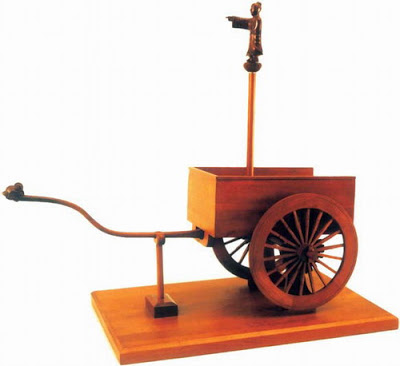
\includegraphics[width=3cm]{./resources/chinesecompasscart.jpg}
					\caption{Chinese Compass Cart}
				\end{figure}
				\column{0.3\textwidth}
				\begin{figure}
					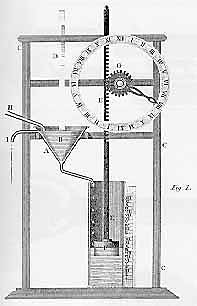
\includegraphics[width=2cm]{./resources/waterclock.jpg}
					\caption{Ctesibius's Water Clock - 300s B.C.}
				\end{figure}
				\column{0.3\textwidth}
				\begin{figure}
					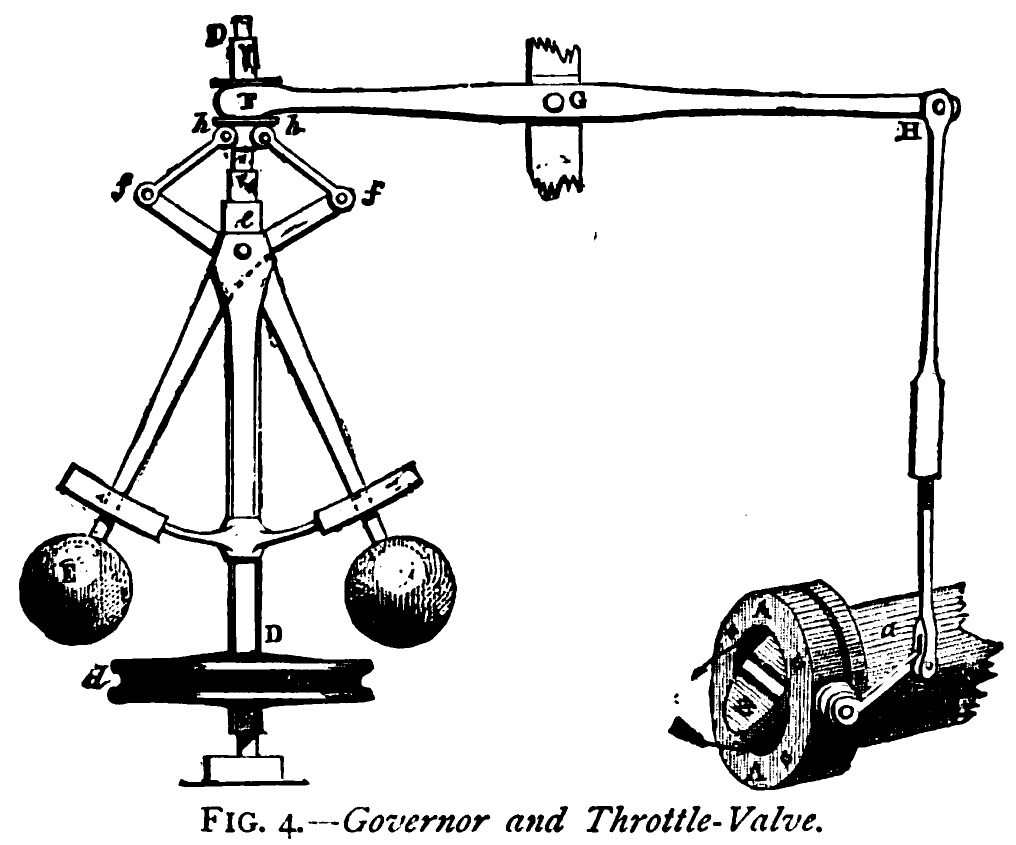
\includegraphics[width=3.5cm]{./resources/flyball.png}
					\caption{James Watt's Flyball Governor - 1780s}
				\end{figure}
			\end{columns}
			\begin{itemize}
				\item<1->All tools incorporated \textcolor{teal}{self-regulating} behavior without so much attention to a specific theory.
			\end{itemize}
		\end{frame}

\section{Proposal}
\subsection{Methodology}
\begin{frame}
\frametitle{Step 1}
\framesubtitle{Overall view}
	\begin{itemize}
		\item<1->The first
		\item<2->The second
		\item<3->The last
	\end{itemize}
\end{frame}
\begin{frame}
\frametitle{Step 1 (Cont'd)}
\framesubtitle{Aspects}
\begin{enumerate}
	\item<1->The first
	\item<2->The second
	\item<3->The last
\end{enumerate}
\end{frame}
\section{References}
	\begin{frame}[t,allowframebreaks]
		\frametitle{References}
		\printbibliography
	\end{frame}

\section*{Appendix}
	\begin{frame}
		\setbeamercovered{transparent}
		\frametitle{Definition(s) of Cybernetics}
		\framesubtitle{Soooo... What is Cybernetics?}
		\begin{itemize}
			\item<1->Ship of the State: The Command of a naval vessel is a metaphor for the governance of a city/state.\\
			--- Plato (420s-340s B.C.)
			\item<2->``Cybernetique is the art of governing or the science of government.''\\
			--- André-Marie Ampère (1775-1836)
			\item<3->``Use the word ‘cybernetics’, Norbert, because nobody knows what it means. This will always put you at an advantage in arguments.''\\
			Widely quoted; attributed to Claude Shannon in a letter to Norbert Wiener in the 1940s.
		\end{itemize}
		\setbeamercovered{invisible}
	\end{frame}

\end{document}

\end{document}